\chapter{Improving Efficiency Using Combined Algorithms}
For our project, we wanted to improve the efficiency of the algorithms in classifying the MET of a signal event as larger than some MET. The way we do this is by determining the thresholds needed to satisfy the trigger rate based on the fraction of background events kept by the trigger system, and then by using those thresholds to compute an efficiency for the same pair of algorithms to classify a signal event as larger than some value of MET.
By signal events, we mean events for which the muon trigger fired, which correspond to events for which a muon was detected.
In this assignment, we wanted to see if we could obtain an increase in efficiency by combining uncorrelated algorithms together subject to the constraint of the trigger rate. The issue is that there are many pairs of thresholds that when combine will keep the proper trigger rate. In the parameter space of all possible combinations of combined thresholds, we have two degrees of freedom in determining what the appropriate thresholds on a pair of algorithms should be. 
In order to simplify the problem, I imposed the constraint that the two trigger rates for the algorithms had to be the same. Therefore, I removed a degree of freedom in the parameter space by constraining my solution space to pairs of thresholds that satisfy the trigger rate and lie on the line $y=x$. The monotonicity of the fraction of events kept as you change either of the thresholds on the algorithms guarantees that there will be a unique solution to both of these constraints on the parameter space. \\
Once we added the constraint of keeping the same fraction individually, the problem essentially became one-dimensional, and I used the popular bisection root-finding method in order to compute the solution to the optimal pair of thresholds. \\
This consisted of guessing an individual fraction for each of the algorithms to keep, and then computing what the combined fraction of events kept was. We iterated this process until the combined fraction kept matched the trigger rate to within one bin.
The level curve describing the set of pairs of thresholds such that the trigger rate constraint is satisfied is given by the constraint:
$$f(\tau_{\alpha},\tau_{\beta})=C$$
for some $C$. Here, $f$ is the function representing the fraction of events kept when the algorithms are used together at the same time. 
This $C$ is determined by the fraction of background events that are kept by the trigger system. 
In order to compute $C$, we used the fraction of passnoalg data that passed an L1 MET cut of $50$ GeV and a CELL MET cut of $100$ GeV. 
For our analysis, $C$ turned out to be $0.0059$.
So we needed to solve the equation $f(\tau_{\alpha},\tau_{\beta})=0.0059$. 
However, because the parameter space is two-dimensional, and the evaluation of $f$ takes a long time (fraction of events kept by both algorithms, and by each one individually), we introduced the constraint that the two individual fractions kept needed to be the same.
In summary, we use the background events in order to compute what the thresholds on the algorithms need to be in order to keep the trigger rate, and then we determine the efficiencies of this combination of algorithms at those thresholds from the signal events. 
\section{Signal Selection on Transverse Mass}
In addition to the cuts on the various algorithms, we also needed to introduce a cut on the transverse mass that is detected to ensure we only keep events with a transverse mass close to that of the W boson ($80.379\pm 0.012 GeV/c^2$). 
We compute the transverse mass using:
$$m_{T}=\sqrt{2P_{\mu}P_{\nu}(1+\cos{(\phi)})}$$
In addition to the previously mentioned cuts, we also added a cut on the transverse mass for the range $40 \leq m_{T} \leq 100$. 
\pagebreak
\section{Results}
\subsection{Algorithms that did not do better combined}
For most pairs of algorithms, we found that combining algorithms such that they keep the correct trigger rate did not yield any gain in efficiency. As in figure \ref{no_gain_efficiency}, we see that the red curve lies underneath the green curve. 
\begin{figure}[h]
        \centering
        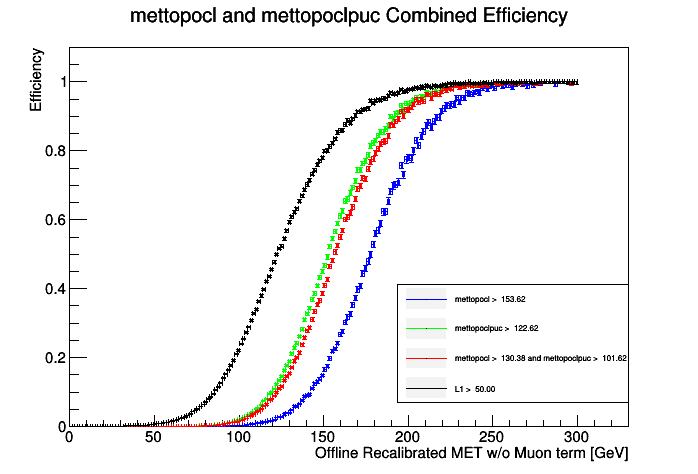
\includegraphics[scale=0.4]{topocl_puc_efficiencies}
        \caption{Efficiencies of METTOPOCL and METTOPOCLPUC}
        \label{no_gain_efficiency}
\end{figure}
\clearpage
\subsection{Algorithms that did do better combined}
We found that we were able to achieve an increase in the overall efficiency for some of the pairs of algorithms considered. 
\begin{figure}[h]
        \centering
        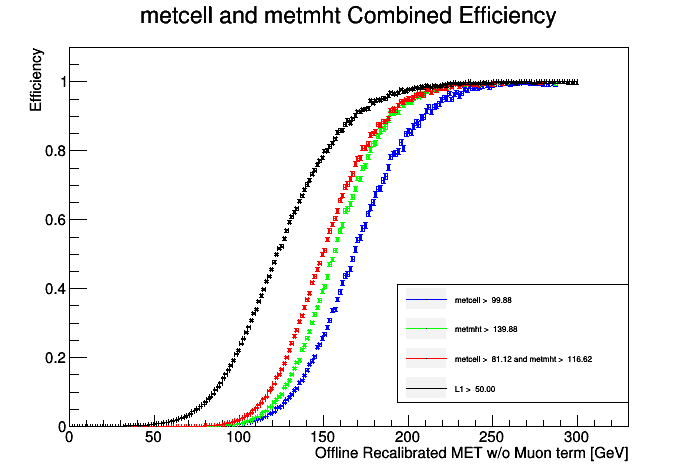
\includegraphics[scale=0.4]{cell_mht_efficiencies}
        \caption{Efficiencies of METCELL and METMHT}
\end{figure}
\begin{figure}[h]
        \centering
        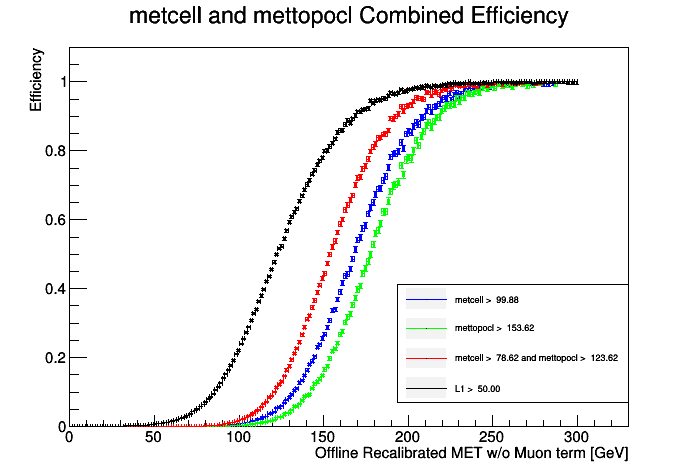
\includegraphics[scale=0.4]{cell_topocl_efficiencies}
        \caption{Efficiencies of METCELL and METTOPOCL}
\end{figure}
\begin{figure}[h]
        \centering
        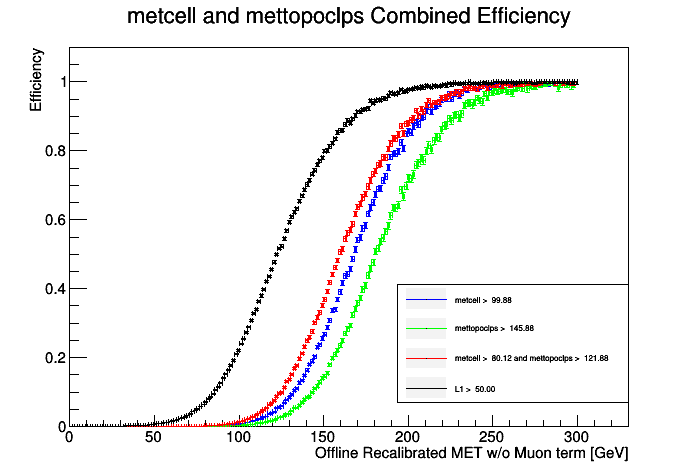
\includegraphics[scale=0.4]{cell_ps_efficiencies}
        \caption{Efficiencies of METCELL and METMHT}
\end{figure}
\begin{figure}[h]
        \centering
        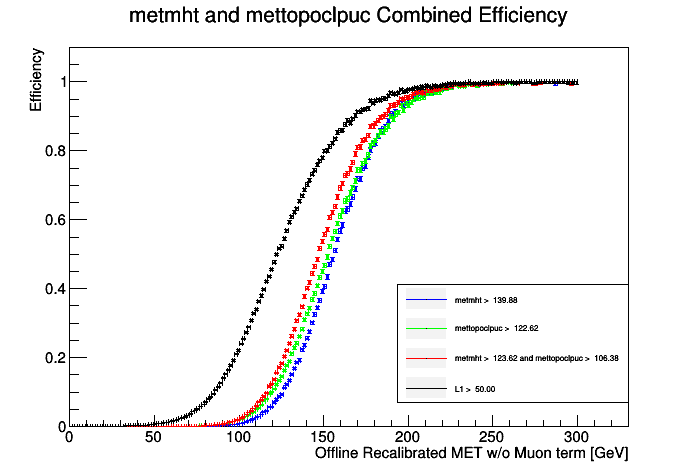
\includegraphics[scale=0.4]{mht_puc_efficiencies}
        \caption{Efficiencies of METCELL and METTOPOCL}
\end{figure}
\clearpage
\subsection{Best Combined Algorithms and Best Individual Algorithms}
During the summer of 2018, the pufit plus cell algorithm trigger was the main one that was actually used for the second part of Run 2.
In figure \ref{bisection_fig}, I've plotted the efficiencies of the best combined algorithms along with the best efficiencies of the individual algorithms. We see that the top curves on this plot are those for combined algorithms, as well as the individual mettopoclpuc and metmht curves.
\begin{figure}[h]
        \centering
        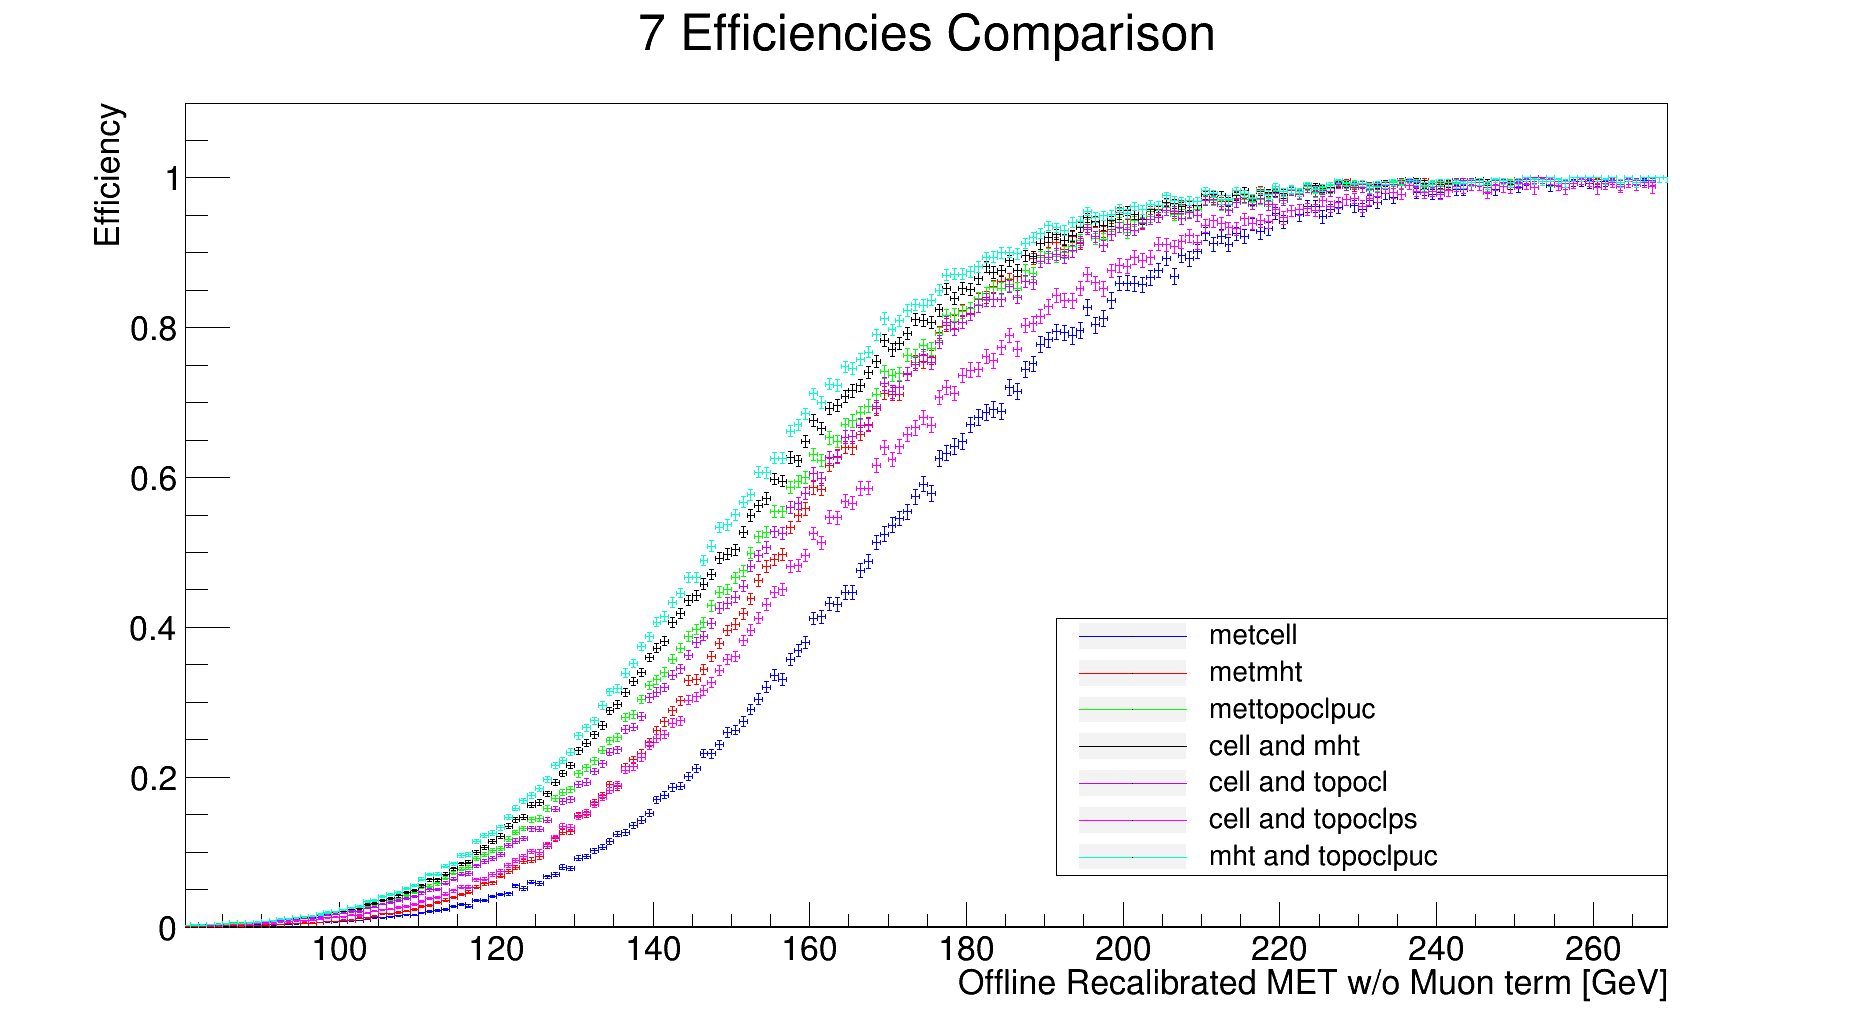
\includegraphics[scale=0.2]{7Efficiencies}
        \caption{Best Combined Efficiency Algorithms Versus Best Individual Algorithms}
        \label{bisection_fig}
\end{figure}
\clearpage
